\chapter{Design and Implementation}
\section{Proposed Architecture}
\subsection{Concepts of DeAr}
\indent 
One of the key features in the DeAr DSP is manipulating Simultaneous Multi-threading (SMT) in each processing core with the purpose of exploiting concurrent arithmetic resources.
By dispatching two instruction streams that manipulate its multi-issue datapath, 
the computational workload of a work-item can be amortized by two threads running simultaneously.
Figure~\ref{fig:bb:1} illustrates the typical execution flow of an HSA work-item across several basic blocks.
A basic block is piece of code without any branch or jump instruction except at its entry or exit.
The life cycle of the work-item involves executing instructions within a block sequentially, and shuttling among the blocks.
DeAr achieves the speedup by exploiting ILP in each basic block, as shown in Figure~\ref{fig:bb:1}. 
At the entry of a program, two DeAr threads are forked by in replacement of a work-item.
Next, the forked DeAr threads simultaneously fetch and execute instructions within the basic block.
They join at the end of the basic block, and perform an identical branch or jump instruction targeting the next basic block simultaneously.
\\\indent
The fundamental challenge in SMT is scheduling for threads, 
which can be resolved by either hardware (dynamic scheduling) or software (static scheduling).
We apply the latter because the static approach offers more optimization opportunities in scheduling, 
and the hardware resources can be dedicated to arithmetics.
\vspace{\textfig}
\begin{figure}[!ht]
    \begin{center}
        \subfigure[Execution flow of an HSA work-item]
        {
            \label{fig:bb:1}
            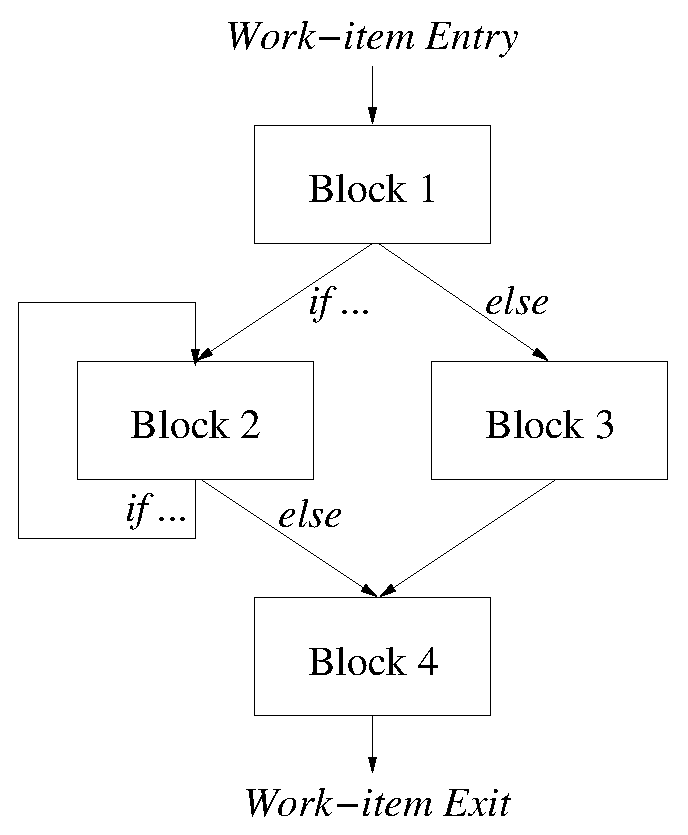
\includegraphics[width=0.3\textwidth]{figs/bb.eps}
        }
        \hfill
        \subfigure[Accelerating the execution of a Basic block]
        {
            \label{fig:bb:2}
            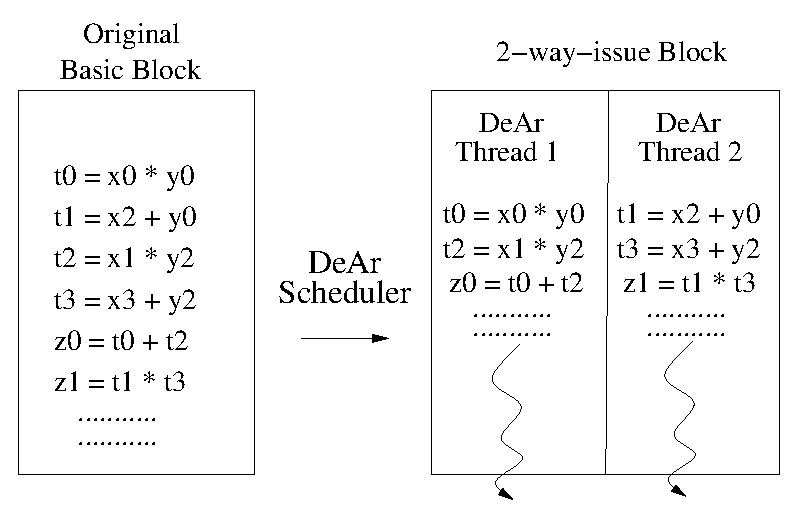
\includegraphics[width=0.55\textwidth]{figs/bb2.eps}
        }
    \end{center}
    \caption{Accelerating HSA with DeAr}
    \label{fig:bb}
\end{figure}
\\\indent 
Another feature of DeAr is exhaustively compacting its datapath while keeping the flexibility and computational power.
This offers DeAr better efficiency in several perspectives including power dissipation, chip area and memory usage.
Moreover, such a compact core design equips it with excellent scalability, 
which makes DeAr suitable for HSA.
A DeAr core can be scaled up to the multi-core architecture, 
where the assembly of cores forms the wavefront which supports the HSA SPMD programming model.
\subsection{System Integration}
\label{sec:integration}
Figure~\ref{fig:archi} illustrates the proposed framework of an HSA system integrated with a 4-core DeAr DSP.
The general purpose processor (GPP) hosts OS and HSA runtime, sharing the main memory with the DeAr DSP.
In the DSP, each core owns a private L1 D-cache, and shared a L1 I-cache with another core.
The L1 I-cache sharing mechanism was proposed in~\cite{kelly2004shared},
which reduces the duplication of program memory in the SPMD model.
The bus interface of the DSP comprises two components, the smart controller (SC) and host port interface (HPI).
SC, proposed by Hsu \textit{et al.}, is a specialized bus interface IP applied to heterogeneous systems.
SC not only performs direct memory access (DMA) for the DSP local memory,
but also re-organize the non-coalescing data transparently to improve the data locality.
On the other hand, HPI, which is a common module found in Texas Instruments DSPs~\cite{hpi},
facilitates the direct access from the GPP to DSP internal resources with purposes below:
\begin{itemize}
    \item \textbf{MMU}: The host OS accesses MMU via HPI, and thus HSA SVM can be facilitated.
    \item \textbf{Dispatch queues}: HSA runtime pushes (pops out) AQL-packets to (from) the kernel-dispatch queue (agent-dispatch queue) via HPI, 
        and thus HSA user-mode queuing can be facilitated.
    \item \textbf{SC}: The SC user API sends control signal to SC via HPI, 
        and thus the data transfer and conversion fashion can be specified by the user.
\end{itemize}

\vspace{\textfig}
\begin{figure}[!ht] 
    \centering
    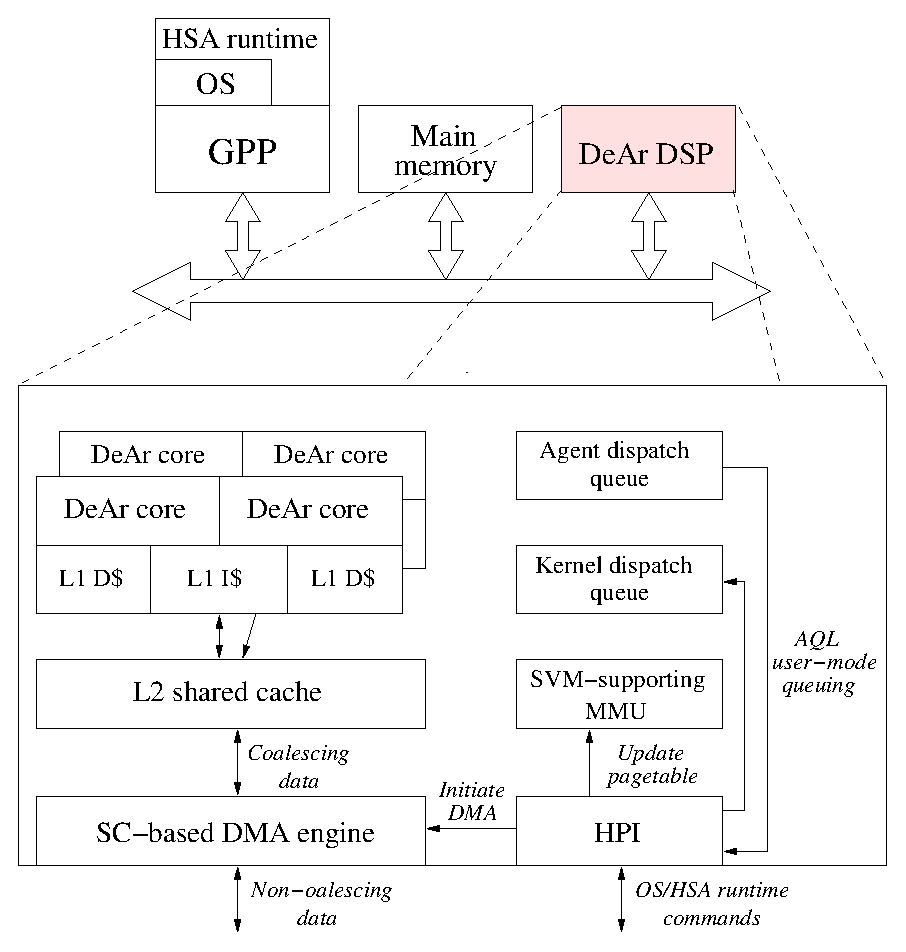
\includegraphics[width=0.8\textwidth]{./figs/archi.eps}
    \caption{Framework for system integration}
    \label{fig:archi}
\end{figure}

\section{Hardware Design and Implementation}
\subsection{Micro-architecture Design}
In this section, we will look into DeAr from a micro-architecture perspective, and explore its design considerations at the same time.
Figure~\ref{fig:micro} illustrates the micro-architecture of DeAr DSP lane.
We adopt the concept of Harvard architecture~\cite{harvard}, 
which separates data memory and instruction memory physically.
As a result, the datapath and the control path are wrapped by two independent interfaces, the load/store (L/S) unit and the instruction unit respectively.
Such orthogonality between data and instructions offers better freedom for optimizing data precision and code density.
The L/S unit supports burst mode transfer, which enables consecutive fetch of the data in the memory.
This mechanism reduces the number of memory access instructions to be used, 
and improve the bus utilization.
In addition, DeAr allows memory transfer to be initiated by two threads orthogonally under the hardware arbitration.
On the other hand, since two DeAr threads always branch simultaneously to the same basic block, 
the compiler can align their simultaneous instructions to adjacent addresses.
As a result, the instruction unit can serve two DeAr threads by doubling the fetch width instead of duplication of the hardware.
\\\indent
Two DeAr threads in a lane share the ALU that commonly exist in a RISC processor.
The demonstrated example includes an adder, a multiplier and a barrel shifter, which are qualified to perform most benchmarks,
Nevertheless, the configuration of the ALU can be customized to fit the target application.
The output of each arithmetic unit connects to an accumulator latch, 
which bypasses the result to ALU inputs.
The bypassing-mechanism of accumulator latches avoids redundant accesses to the RF, 
and thus reduces the power dissipation in the RF.
Besides, DeAr can preserve the data in an accumulator latch until the corresponding arithmetic unit is activated again, 
offering more data bypassing opportunities.
The bypassing mechanism and resolution of structural hazards are both handled by the software to reduce hardware complexity.
\\\indent
The RF is physically and symmetrically divided for two DeAr threads.
Each of them owns a pair of queue memory module as well as a stack memory module, 
and these memory units form the sequential-accessed banked register file (SBRF).
The banked organization of SBRF cuts off redundant connectivity among read/write ports and register cells.
Compared with the conventional centralized organization, 
its wire area and power dissipation are significantly improved.
A load-queue and a store-queue serve as the buffer that connects the lower level of the memory hierarchy with the datapath.
They can be accessed from their both sides concurrently in the first-in-first-out (FIFO) fashion.
A DeAr thread reads input data from its load-queue and writes computation results to its store-queue, 
while the L/S unit accesses queues in the opposite direction against the dataptah.
By preventing queues from empty or full with clever scheduling, the latency of L/S can thus be hidden.
The stack memory, on the other hand, is responsible for the storage of intermediate data and L/S address.
Other possible uses of the stack memory include branch condition evaluation and returning from interruptions.
The access pattern of a stack memory is last-in-first-out (LIFO), 
which is the key feature of the HDFG-base scheduling elaborated in Section\ref{sec:scheduling}.
Applying sequential-access memory modules instead of random-access ones effectively reduces the control signal size and decode overhead, 
since any access to the SBRF can be simplified to "PUSH" or "POP".
Such simplification gains high code density and save the wiring from the instruction unit to SBRF, 
and constitutes the key advantage of DeAr over conventional VLIW architectures.
For clarity, we summarize the classification of various registers/latches in the datapath in Table~\ref{tab:register}.
\begin{table}[!ht]
    \caption{Classification of data registers/latches in DeAr}
    \label{tab:register}
    \centering
    \begin{tabular}{|l|l|l|}
        \hline
        \multicolumn{1}{|c|}{\textbf{Register type}} & \multicolumn{1}{c|}{\textbf{Dedicated to}} & \multicolumn{1}{c|}{\textbf{Description}}                 \\ \hline
        Load-queue                                   & \multirow{3}{*}{a DeAr thread}             & buffers input data received from the main memory          \\ \cline{1-1} \cline{3-3} 
        Store-queue                                  &                                            & buffers output data sent to the main memroy               \\ \cline{1-1} \cline{3-3} 
        Stack                                        &                                            & buffers intermediate data of computation                  \\ \hline
        Accumulator                                  & an arithmetic unit                         & buffers the arithmetic result of the previous clock cycle \\ \hline
    \end{tabular}
\end{table}
\\\indent
The design of transport triggered data bus (TTDB) was inspired by TTA~\cite{move}.
TTDB separates the RF from the ALU with a set of multiplexers controlled by the instruction unit, 
and bypasses data from accumulators.
Possible routes of data over TTDB are summarized as below:
\begin{itemize}
    \item Each arithmetic unit receives the first operand from a load-queue or an accumulator, 
        and receives the second one from a load-queue or a stack.
    \item Each store-queue receives data from the output of an arithmetic unit.
    \item Each stack receives data from the output of an arithmetic unit.
\end{itemize}
\indent
It is important to note that, even though the communication among the RF, ALU and accumulators is compacted exhaustively, 
the datapath flexibility is still kept.
The organization of TTDB is tightly coupled with the instruction set architecture (ISA).
Accordingly, further reduction in code size can be achieved with such a compact design.
More insight into the relation between TTDB and ISA is available in Section~\ref{sec:isa}.

\vspace{\textfig}
\begin{figure}[!ht] 
    \centering
    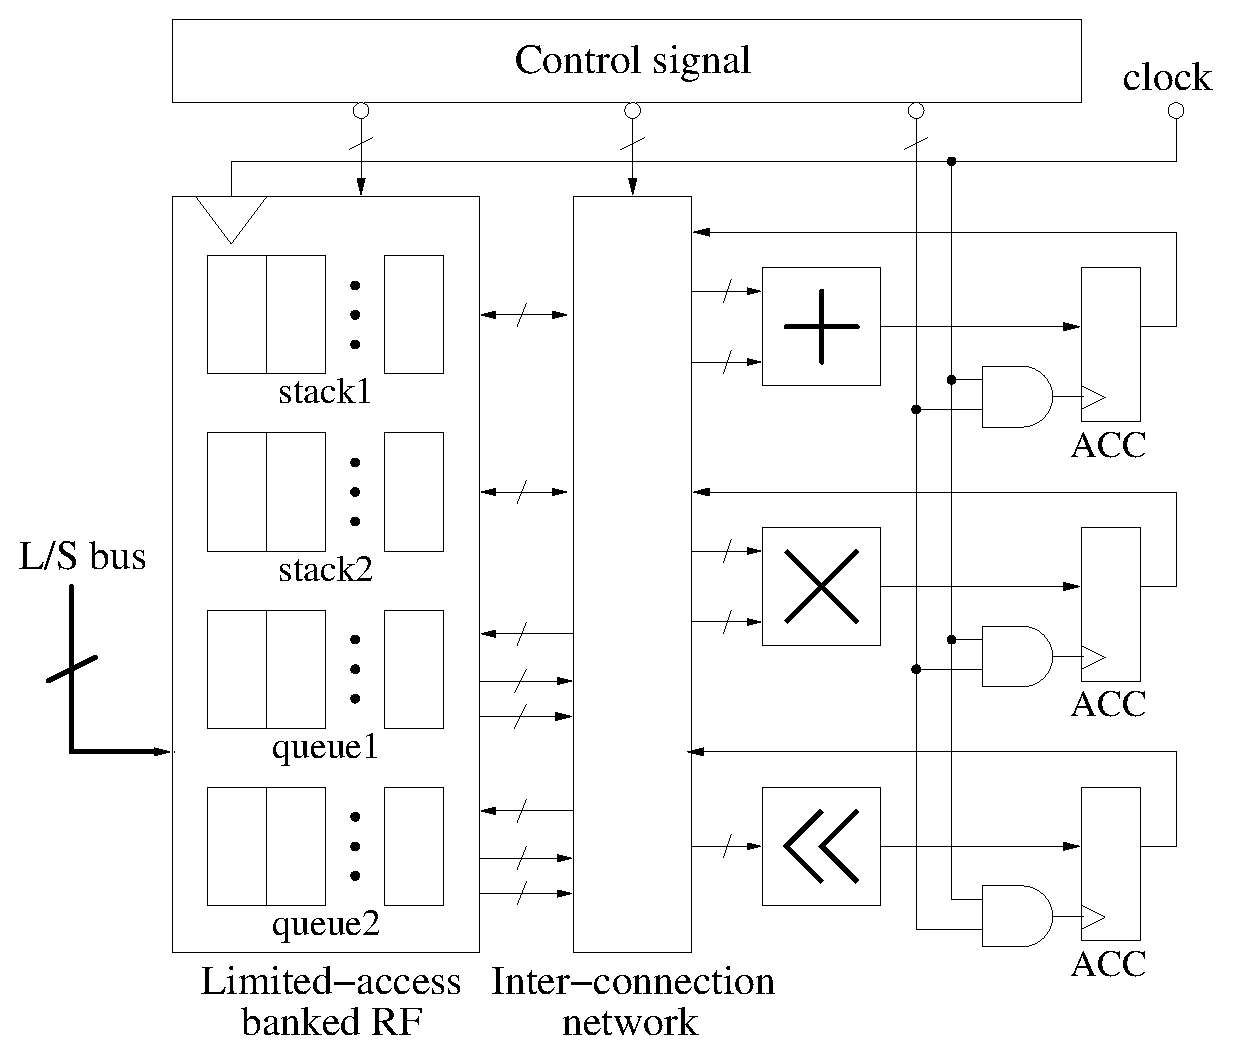
\includegraphics[width=0.85\textwidth]{./figs/micro.eps}
    \caption{Micro-architecture of a DeAr DSP lane}
    \label{fig:micro}
\end{figure}


\subsection{Instruction Set Architecture}
\label{sec:isa}
\indent The DeAr instruction set architecture (ISA) seemingly follows the principle of RISC, which takes instructions with fixed length, 
but the former is optimized for efficient arithmetic.
Each DeAr instruction is composed of two portions, RISC-style portion and stack-access portion.
%The instruction unit issues two instructions simultaneously for two DeAr threads.
Table~\ref{tab:risc} shows the functions of the RISC-style portion, which are similar to the subset of RISC ISA.
Here, we use the bold alphabets, \textbf{r}, \textbf{s}, \textbf{t}, \textbf{k}, \textbf{a}, 
to represent the instruction decode bit-fields and illustrate the meaning of each function.
According to their functions, they can be classified to three categories, A-type, B-type and M-type.
The A-type includes arithmetic instructions such as addition (ADD or SUB), multiplication (MUL) and shift operation (SHL or SHR).
Other instructions like move (MV), which moves data from the other DeAr thread, 
and no operation (NOP), which stalls the DeAr thread for a cycle, 
belong to the A-type as well since they manipulate the datapath in a similar way.
The B-type includes instructions which interact with the instruction unit, such as branch on zero (BE), branch on nonzero (BNE) and unconditional branch (JMP).
The M-type, on the other, includes memory transfer instructions, load (LD) and store (ST), which manage the load/store unit.
%---------- risc-style portion table
\begin{table}[ht!]
    \centering
    \caption{RISC-style portion of the DeAr instruction set}
    \label{tab:risc}
    \begin{tabular}{|c|l|l|c|}
        \hline
        \multicolumn{1}{|c|}{\textbf{Category}} & \multicolumn{1}{c|}{\textbf{Name}} & \multicolumn{1}{c|}{\textbf{Meaning}} & \multicolumn{1}{c|}{\textbf{Target}} \\ \hline
    \multirow{7}{*}{ \begin{tabular}[c]{@{}l@{}} \\ A type \end{tabular}}      & ADD & \textbf{d} = \textbf{s} + \textbf{t}  & \multirow{7}{*}{\begin{tabular}[c]{@{}l@{}} \\ Datapath \end{tabular}}  \\ \cline{2-3}
                                                                               & SUB & \textbf{d} = \textbf{s} - \textbf{t} & \\ \cline{2-3} 
                                                                               & MUL & \textbf{d} = \textbf{s} * \textbf{t} & \\ \cline{2-3} 
                                                                               & SHL & \textbf{d} = \textbf{s} << \textbf{t} & \\ \cline{2-3}
                                                                               & SHR & \textbf{d} = \textbf{s} >> \textbf{t} & \\ \cline{2-3}
                                                                               & MV  & \textbf{d} = \textbf{s} + 0 or \textbf{d} = \textbf{s} << 0 & \\ \cline{2-3} 
                                                                               & NOP & \begin{tabular}[c]{@{}l@{}}1. disable write back \\ 2. clock-gate the accumulator \end{tabular}& \\ \hline
    \multirow{3}{*}{ \begin{tabular}[c]{@{}l@{}} \\ \\ B type \end{tabular}}          & JMP & pc = pc + \textbf{a}  & \multirow{3}{*}{ \begin{tabular}[c]{@{}l@{}} \\ \\ Instruction unit \end{tabular}} \\ \cline{2-3}
                                                                                      & BZ  & \begin{tabular}[c]{@{}l@{}} \textit{if}(stack1.read() == stack2.read())\\ \ \ \ \ \ \ \ pc = pc + \textbf{a} \end{tabular} & \\ \cline{2-3}
                                                                                      & BNZ & \begin{tabular}[c]{@{}l@{}} \textit{if}(stack1.read() != stack2.read())\\ \ \ \ \ \ \ \ pc = pc + \textbf{a} \end{tabular} & \\ \hline
    \multirow{2}{*}{ \begin{tabular}[c]{@{}l@{}} \\ M type \end{tabular}}           & LD  & \begin{tabular}[c]{@{}l@{}} \textit{repeat}(\textbf{r})\\ \ \ \ \ \ \ \ load\_queue.push (memory[\textbf{a}]) \end{tabular}& \multirow{2}{*}{\begin{tabular}[c]{@{}l@{}} \\  Load/store unit \end{tabular}} \\ \cline{2-3} 
                                                                                    & ST  & \begin{tabular}[c]{@{}l@{}} \textit{repeat}(\textbf{r})\\ \ \ \ \ \ \ \ memory[\textbf{a}] = store\_queue.pop() \end{tabular}& \\ \hline
    \end{tabular}
\end{table}
%-----------------------------------------

\indent 
On the other hand, the stack-access portion, illustrated in Table~\ref{tab:stack}, 
is dedicated to the manipulation of the stack memory.
Four stack operations, \textit{PUSH}, \textit{POP}, \textit{MODIFY} and \textit{STALL}, are defined, 
Each DeAr thread uses these stack operations to buffer its intermediate data in the LIFO-manner.
A \textit{PUSH} stores the result from one of arithmetic units and adds the head address by 1, 
while a \textit{POP} eliminates the head data by subtracting the head address by 1.
Since a \textit{PUSH} following a \textit{POP} modifies the head data and cancels the address decrement, 
a \textit{MODIFY} is defined to simplify the combination the operations.
In some scenarios, a DeAr thread does nothing to the stack but keeps its status.
As a result, a \textit{STALL} is also defined for the stack-access portion.
These two portions compose DeAr ISA.
Each DeAr thread can thus access an arithmetic unit with the RISC-style portion and handle the intermediate data with the stack-access portion.
On the other hand, since the memory transfer instructions (i.e., LD and ST) never generate intermediate data, 
their stack-access portion is set to \textit{STALL} implicitly.
We can thus preserve more bits in the memory transfer instruction to address more memory space.

%---------- stack portion table
\begin{table}[ht!]
    \centering
    \caption{Stack access portion of the DeAr instruction set}
    \label{tab:stack}
    \begin{tabular}{|l|l|l|}
        \hline
        \multicolumn{1}{|c|}{\textbf{Name}} & \multicolumn{1}{c|}{\textbf{Meaning}} & \multicolumn{1}{c|}{\textbf{Note}} \\ \hline
    PUSH & \begin{tabular}[c]{@{}l@{}}1. Add the head address by 1\\ 2. Write the new data to the head address\end{tabular} & \multirow{2}{*}{ \parbox{5cm}{A "pop" followed by a "push" is equivalent to a "modify"} } \\ \cline{1-2}
    POP                               & \begin{tabular}[c]{@{}l@{}}1. Subtract the head address by 1\\ 2. Invalidate the previous head data\end{tabular} & \\ \hline
        MODIFY                            & Modify the head data to to the new data & The head address remains \\ \hline
        STALL                               & No operation & The head address and data remain \\ \hline
    \end{tabular}
\end{table}
%-----------------------------------------

Each DeAr instruction is 12-bit in length.
To offer better insight into the instruction decode mechanism, 
Table~\ref{tab:decode} elaborates three instruction types, 
each of which is enumerated from its MSB to LSB.
Marks of the first column represent various bit-fields, 
and they correspond to the bold alphabets shown in Table~\ref{tab:risc}.
%Note that Table~\ref{tab:decode} also reveals the detailed organization of the TTDB by elaborating the communication in the datapath.
\\\indent
A-type instructions include all arithmetic instructions.
The head 4-bit \textbf{f}, which is similar to the function code in RISC, specifies the operation to be performed.
It is followed by a single-bit signal \textbf{d}, which determines whether the result of this operation is written back to the memory via the store-queue.
After that, a pair of 2-bit, \textbf{s} and \textbf{t}, select the sources of two arithmetic operands respectively. 
Nevertheless, the data sources selected by \textbf{s} and \textbf{t} are not identical.
The former selects the first operand from the load-queue or one of accumulators, 
while the latter selects the second operand from the load-queue, stack, or constants (1 or 0).
Some instructions like SHR and SHL use immediate data as the second operand (i.e., shifting amount).
In such a scenario, \textbf{t} and the reserved bit serve as immediate data.
Finally, the last 2-bit \textbf{k} is the stack access portion, which encodes four operations that manipulate the stack memory.
Note that functions of \textbf{f} and \textbf{k} remain in the M-type and B-type.
\\\indent 
On the other hand, M-type instructions perform memory transfers.
The function field \textbf{f} is followed by 2-bit \textbf{w}, 
which specifies the word size of the transfer.
The size can be byte (8-bit), halfword (16-bit) or word (32-bit).
Another bit \textbf{b} indicates whether the memory transfer is performed in the burst mode, 
and the following 2-bit \textbf{r} determines the length of the burst (i.e., the number of transfers to be performed consecutively).
The burst length can be 2, 4, 8 or 16.
If \textbf{b} is de-asserted, \textbf{r} will be ignored.
\\\indent 
The last category, B-type instruction, which controls the program flow, 
is a special case compared with the other two types.
Since two DeAr threads always perform identical branch instructions synchronously, 
two branch instructions can be merged into one with more bits for branch target addressing.
As a result, B-type instructions can manipulate 24-bit, which is twice of the original one in length.
The function field \textbf{f} is thus followed by 16-bit branch address offset \textbf{a}.
%Likewise, the last 2-bit \textbf{k} denotes the stack access portion, which follows unused 2 bits.

%---------- bit field table---------------
\begin{table}[!ht]
    \centering
    \caption{Instruction decode table of the DeAr ISA}
    \label{tab:decode}
    \begin{tabular}{|l|l|l|}
        \hline
        \multicolumn{1}{|c|}{\textbf{Mark}} & \multicolumn{1}{c|}{\textbf{Bit field}} & \multicolumn{1}{c|}{\textbf{Description}} \\ \hline
        \multicolumn{3}{|c|}{\textbf{A-type instructions}} \\ \hline
    f & {[}11:8{]} & \begin{tabular}[c]{@{}l@{}}Select the function from ADD, SUB, SHL, SHR, MUL, MV or NOP\end{tabular} \\ \hline
    d & {[}7{]} & \begin{tabular}[c]{@{}l@{}}Enable WB to the store-queue\end{tabular} \\ \hline
    s & {[}6:5{]} & \begin{tabular}[c]{@{}l@{}}Select the first operand from load-queue or accumulators \end{tabular} \\ \hline
    t & {[}4:3{]} & \begin{tabular}[c]{@{}l@{}}1. Select the second operand from load-queue, stack, constant 0 or 1 \\ 2. Immediate data for SHR or SHL\end{tabular} \\ \hline
    - & {[}2{]} & \begin{tabular}[c]{@{}l@{}}1. Reserve \\ 2. Immediate data for SHR or SHL\end{tabular} \\ \hline
    k & {[}1:0{]} & \begin{tabular}[c]{@{}l@{}}Stack access portion\end{tabular} \\ \hline
        \multicolumn{3}{|c|}{\textbf{M-type instructions}} \\ \hline
    f & {[}11:8{]} & \begin{tabular}[c]{@{}l@{}}Select the function from LD or ST\end{tabular} \\ \hline
        %e & {[}7{]} & \begin{tabular}[c]{@{}l@{}}Specify the endianness of the data in the memory \end{tabular} \\ \hline
    w & {[}7:6{]} & \begin{tabular}[c]{@{}l@{}}Select the word size from byte, halfword or word \end{tabular} \\ \hline
    b & {[}5{]} & \begin{tabular}[c]{@{}l@{}}Enable burst mode memory transfer \end{tabular} \\ \hline
    r & {[}4:3{]} & \begin{tabular}[c]{@{}l@{}}Select the burst length from 2, 4, 8 or 16 \end{tabular} \\ \hline
    - & {[}2{]} & \begin{tabular}[c]{@{}l@{}}Reserve \end{tabular} \\ \hline
    k & {[}1:0{]} & \begin{tabular}[c]{@{}l@{}}Stack access portion\end{tabular} \\ \hline
        \multicolumn{3}{|c|}{\textbf{B-type instructions}} \\ \hline
    f & {[}23:20{]} & \begin{tabular}[c]{@{}l@{}}Select the function from BE or BNE\end{tabular} \\ \hline
    a & {[}19:4{]} & \begin{tabular}[c]{@{}l@{}}Specify the branch address offset \end{tabular} \\ \hline
    - & {[}3:2{]} & \begin{tabular}[c]{@{}l@{}}Reserve \end{tabular} \\ \hline
    k & {[}1:0{]} & \begin{tabular}[c]{@{}l@{}}Stack access portion\end{tabular} \\ \hline
    \end{tabular}
\end{table}
%------------------------------------------


\section{Software Design and Implementation}
\label{sec:software}
\subsection{Software framework for DeAr}
\label{sec:swframework}
To fully exploit the power of DeAr, we also present a complete code generation flow including compilation, scheduling and optimization.
Algorithm~\ref{alg:framework} provides an overview of the software framework for DeAr. 
The user only needs to provide DSP kernel code written in OpenCL, and a flag indicating the code optimization level.
With CLOC \cite{cloc} tool provided by \textit{HSA Foundation}, the kernel code is converted to standardized HSAIL, $H$, as shown in Line~\ref{line:tohsail}.
Next, in Line~\ref{line:trans}--\ref{line:trane}, 
we run the HSAIL transformation (Section~\ref{sec:trans}) on HSAIL code and obtain a hierarchical data flow graph (HDFG), 
$\bar{G}$ (Section~\ref{sec:hdfg}), which holds crucial scheduling heuristics.
After that, Line~\ref{line:optstart} to \ref{line:optend} perform the key part of DeAr software, 
operation scheduling and optimization (Section~\ref{sec:scheduling}).
The optimization flag $\lambda$ in Line~\ref{line:forlambda} determines the number of iterations to be used.
For each iteration, the scheduler exhausts heuristics in $\bar{G}$ which optimize the cycle and WB counts with certain randomness.
Finally, the scheduler selects the best scheduling result $C_{golden}$ among iterations and generates the final code $X_{golden}$ for as the output.
%-----------------framework algo -------------
\begin{algorithm}[h]
    \caption{\textproc{Software Framework for DeAr}}
    \begin{algorithmic}[1]
        \Require 
        High-level DSP kernel code in OpenCL, Optimization flag $\lambda$
        \Ensure 
        Binary code of DeAr

        %\State Convert the kernel code to HSAIL code
        \State $hsail \Leftarrow$ \Call{CL Offline Compiler }{ $kernel$ }
        \label{line:tohsail}
        %\State Perform SSA transformation on HSAIL;
        %\label{tossa}
        %\State Convert SSA code to DFG, $G = ( V_{op} , E_{op} )$, where $V_{op}$ is the set of operations and $E_{op}$ is the set of their dependencies;
        %\label{todfg}
        %\State Perform hierarchization on $G$, and get $\bar{G} = ( V_{bt} , E_{bt} )$, where $V_{bt}$ is a set of binary trees and $E_{bt}$ is the set of their dependencies;
        \State $G \Leftarrow$ \Call{Convert HSAIL to DFG by SSA }{ $hsail$ }
        \label{line:trans}
        \State $\bar{G} \Leftarrow$ \Call{Hierarchize DFG to HDFG }{ $G$ }
        %\State Perform the HSAIL transformation on HSIL code, and obtain a HDFG, $\bar{G}$
        \label{line:trane}
        \State $C_{golden} \Leftarrow  \infty$
        \label{line:optstart}
        \For {$i=1$ to $f(\lambda)$}
        \label{line:forlambda}
        %\State Schedule operations in $\bar{G}$ and get binary code $X_i$ and its total cycle count $C_i$
        %\State $X_{inter}, bt_{remain} \Leftarrow$ \Call{Inter-tree Scheduling }{ $\bar{G}$ }
        \State $X_i, C_i \Leftarrow$ \Call{HDFG-based Scheduling }{ $\bar{G}$ }
        \If {$C_i < C_{golden}$}
        \State $C_{golden} \Leftarrow C_i$
        \State $X_{golden} \Leftarrow X_i$
        \EndIf
        \EndFor
        \State Return $X_{golden}$
        \label{line:optend}
    \end{algorithmic}
    \label{alg:framework}
\end{algorithm}
%-----------------------------------------

\subsection{Data Flow Graph and Hierarchical Data Flow Graph}
\label{sec:hdfg}
A data flow graph (DFG), which presents dependencies among operations, is crucial information for program analysis.
By partitioning a program into basic blocks, the control flow can be simplified, and thus each DFG of a basic block is a directed acyclic graph (DAG).
Figure~\ref{fig:dfg:dfg} illustrates an example of a DFG, where each node and each edge denote an operation and a dependency respectively.
We can further express any DFG as a data structure $G$, which holds a set of nodes (operations), $V_{op}$, and a set of edges (dependencies), $E_{op}$
In conventional DSP compiler design, optimal scheduling of operations is often approached by analyzing the DFG.
For example, \cite{dsplite} solves ILP problems \cite{ilp} in a DFG to approximate optimal scheduling, 
and the list scheduling \cite{list} calculates the scheduling range of each operation in a DFG as the scheduling criterion. 
\\\indent
However, we noticed that the conventional DFG analysis is infeasible for DeAr due to its datapath uniqueness.
As a result, in this work, we propose an enhanced version of the DFG, the hierarchical data flow graph (HDFG), which fits DeAr.
Figure~\ref{fig:dfg:hdfg} demonstrates the HDFG, $\bar{G} = {V_{bt}, E_{bt}}$, converted from Figure~\ref{fig:dfg:dfg}.
We enumerate several important features of the HDFG as below: 
\begin{itemize}
    \item Cascaded operations ($op$) form a super node ($sn$), and an isolated $op$ forms a $sn$ directly. 
Within a $sn$, an $op$ forwards data to the next one.
    \item Neighboring $sn$s form a full binary tree ($bt$), and isolated $sn$ forms a $bt$ directly.
These $bt$s further form a set of vertices, $V_{bt}$.
Within a $bt$, a parent $sn$ receives the first operand popped from the stack and the second one forwarded via TTDB.
    \item Dependencies among $op$s that cross $bt$s are inherited by the $bt$s they belong to.
These inherited dependencies form a set of edges, $E_{bt}$, of $V_{bt}$.
    \item A $bt$ without any in-edge existing in $\bar{G}$ (i.e., $bt \in V_{bt}\ |\ \textrm{deg}^-(bt) = 0$) is free to be scheduled. 
After scheduled, the $bt$ and its edges are erased from the $\bar{G}$.%
\end{itemize}

\indent The hierarchy of HDFGs provides crucial optimization information to the DeAr scheduler.
The scheduler eliminates redundant RF access within each $sn$, and regularize the RF access pattern into stack's FILO-fashion by manipulating the recursive property of each $bt$.
Moreover, the binary property of $bt$ also provides more opportunities for balancing workload of two threads, and thus ILP is achieved.
\vspace{\textfig}
\begin{figure}[!ht]
    \begin{center}
        \subfigure[DFG example]
        {
            \label{fig:dfg:dfg}
            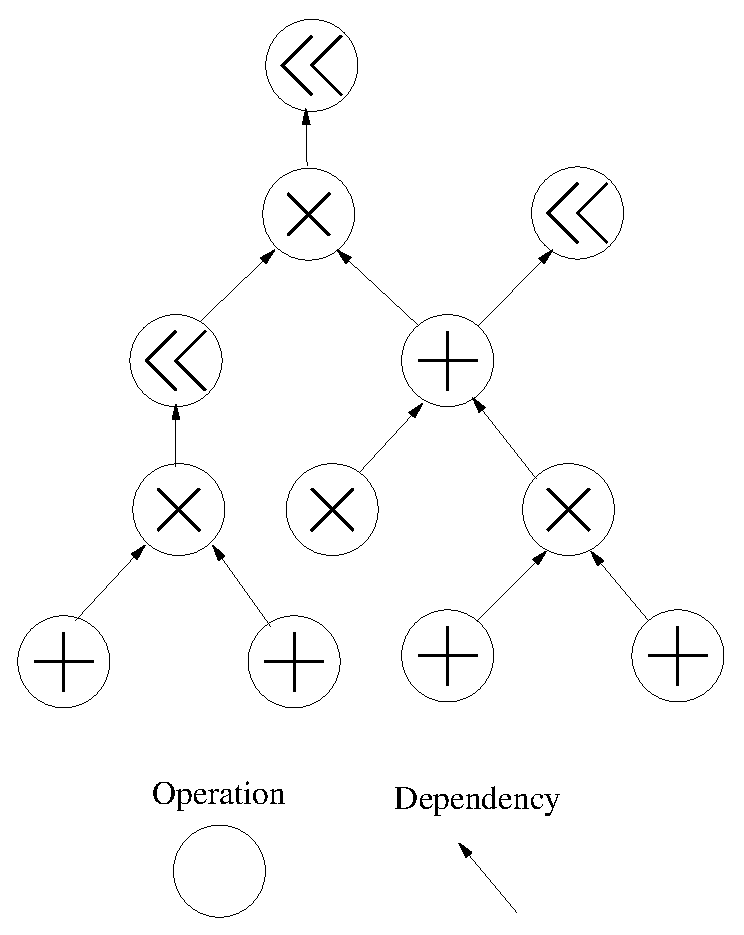
\includegraphics[width=0.45\textwidth]{figs/dfg.eps}
        }\hfill
        \subfigure[Corresponding HDFG]
        {
            \label{fig:dfg:hdfg}
            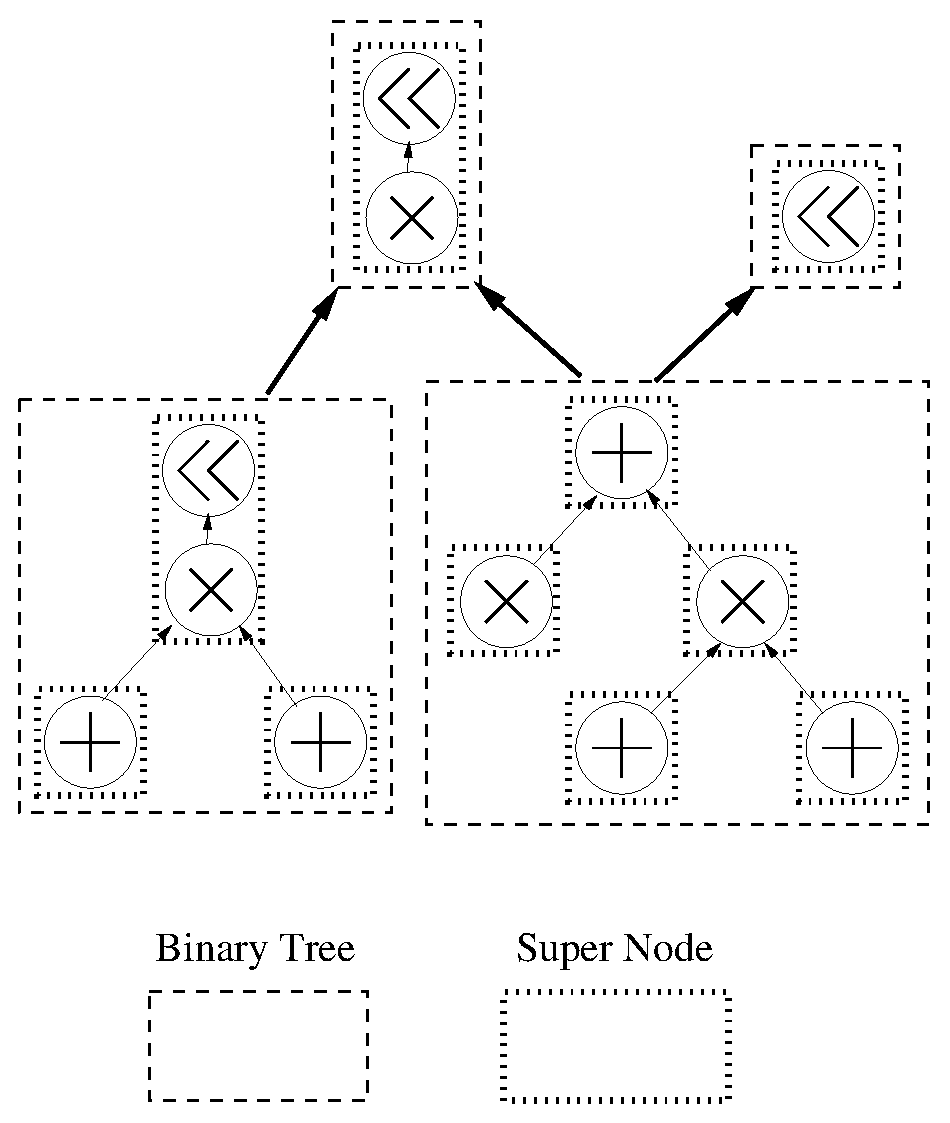
\includegraphics[width=0.45\textwidth]{figs/hdfg.eps}
        }
    \end{center}
    \caption{Conversion from DFG to HDFG}
    \label{fig:dfg}
\end{figure}


\subsection{HSAIL Transformation}
\label{sec:trans}
The whole process of the HSAIL transformation contains two phases elaborated as below:
\begin{itemize}
    \item \textbf{Phase-1: Convert HSAIL to DFG by SSA} \\\indent
        Details of the first phase is shown in Algorithm~\ref{alg:2dfg}.
        Single static assignment (SSA)~\cite{ssa} is a popular form of IR which simplifies the work of compiler, 
        and thus deriving the SSA form of the code becomes the first step.
        SSA form specifies that each variable must be assigned exactly once, which is the key distinction from HSAIL.
        %\\\indent
        The conversion from normal HSAIL to SSA form is initialized by performing reaching definition analysis \cite{rda} as shown in Line~\ref{line:rda}.
        Next, for each assignment in the code, we give a new name to the LHS variable, and update corresponding new names of RHS variables indicated by reaching definition analysis.
        These iterations deriving the SSA form correspond to Line~\ref{line:forhsails}--\ref{line:forhsaile}.
        Now, each assignment to some variable $X$ denotes an operation, which dominates operations with $X$ appearing in their RHS variables.
        As a result, we can construct the DFG without burden by iterating the new code, as shown in Line~\ref{line:forssas}--\ref{line:forssae}.
        Operations and their dependencies are stored in a set of vertices $V_{op}$ and a set of edges $E_{op}$ respectively, 
        and thus the DFG, $G = ( V_{op} , E_{op} )$, is constructed.
        %----------hsail to dfg algo--------------
        \begin{algorithm}[ht!]    \caption{\textproc{Convert HSAIL to DFG by SSA}}
            \begin{algorithmic}[1]
                \Require    HSAIL code
                \Ensure     $G = ( V_{op} , E_{op} )$   \Comment{ DFG }
                \State      Peform reaching definition analysis     \label{line:rda}
                \For        {each assignment (operation) in the HSAIL code}     \label{line:forhsails}
                \State      Give a new name to the LHS variable
                \State      Update RHS variables with corresponding new names in other assignments
                \EndFor                                                     \label{line:forhsaile}
                \State      Initialize $G \textrm{, where } V_{op} = \emptyset \textrm{ and } E_{op} = \emptyset $
                \For        {each assignment (operation) in the new HSAIL code} \label{line:forssas}    \Comment{SSA form}
                \State      Insert the LHS variable $x$ to $V_{op}$
                \For        {each variable $y$ in the RHS}
                \State      Insert a new edge ($x$, $y$)
                \EndFor
                \EndFor                                                         \label{line:forssae}
            \end{algorithmic}
            \label{alg:2dfg}
        \end{algorithm}
        %----------------------------------------

    \item \textbf{Phase-2: Hierarchize DFG to HDFG} \\\indent
        %As discussed in~\ref{sec:hdfg}, the HDFG is an enhanced version of the DFG which provides necessary heuristics for DeAr scheduler.
        Hierarchizing the DFG to the HDFG is achieved by traversing the former, and its details are shown in Algorithm~\ref{alg:tohdfg}.
        In Line~\ref{line:forroots}--\ref{line:forroote}, the algorithm firstly iterates all root operations (i.e., $\textrm{deg}^+(op)=0$ ) in $G$,
        and call the first subroutine, \textproc{Build Binary Tree }, on each root operations.
        Line~\ref{line:bbts}--\ref{line:bbte} show the details of \textproc{Build Binary Tree }.
        A binary tree $bt$ is initialized by building a super node $sn$ on the input operation $op$ with the second subroutine, \textproc{Build Super Node }, which groups cascaded operations ending with $op$, as shown in Line~\ref{line:bsns}--\ref{line:bsne}.  After that, the third subroutine \textproc{Grow Binary Tree }, described in Line~\ref{line:gbts}--\ref{line:gbte}, will expand $bt$ by including neighboring operations if each $op$ has exactly one out-edge (i.e., $\textrm{deg}^+(op)=1$), as shown in Line~\ref{line:growifs}--\ref{line:growife}.  \\\indent On the contrary, if the aforementioned condition is not met with any of $op_{left}, op_{right}$, 
        it will call \textproc{Build Binary Tree } on both to build new binary trees, $bt_{left}, bt_{right}$,
        and record the new dependencies, $bt_{left} \rightarrow bt, bt_{right} \rightarrow bt$.
        This step is demonstrated in Line~\ref{line:growelses}--\ref{line:growelsee}. 
        %\\\indent
        The recursion proceeds by cross-calling between \textproc{Build Binary Tree } and \textproc{Grow Binary Tree } until the whole DFG is traversed.
        Binary trees and their dependencies are stored in a set vertices $V_{bt}$ and a set of edges $E_{bt}$ respectively.
        Finally, the HDFG, $\bar{G} = ( V_{bt} , E_{bt} )$, is constructed and returned.
\end{itemize}

%----------DFG to HDFG algo--------------
\begin{algorithm}[ht!]    \caption{\textproc{Hierarchize DFG to HDFG}}
    \begin{algorithmic}[1]
        \Require    $G = ( V_{op} , E_{op} )$ \Comment{ DFG }
        \Ensure     $\bar{G} = ( V_{bt} , E_{bt} )$ \Comment{ HDFG }
        \State      Initialize $\bar{G} \textrm{, where } V_{bt} = \emptyset \textrm{ and } E_{bt} = \emptyset $
        \For        {each of $  op \ni \sum_{op \in V_{op}}\textrm{deg}^+(op) = 0 $}  \label{line:forroots}   \Comment{For each root vertex}
        \State      $v_{bt} \Leftarrow $\Call{Build Binary Tree }{$op$}
        \State      Insert $v_{bt}$ to $V_{bt}$
        \EndFor                                                                    \label{line:forroote}
        \Statex %---------------------------
        \Function   {Build Binary Tree }{$op$}         \label{line:bbts}
        \State      Initialize a birary tree $bt$
        \State      $sn \Leftarrow$ \Call{Build Super Node }{$op$}
        \State      Set $sn$ as the root of $bt$
        \State      \Call{Grow Binary Tree }{$sn$}
        \State      \Return {$bt$}
        \EndFunction                                \label{line:bbte}
        \Statex %--------------------------
        \Function   {Grow Binary Tree }{$sn$}          \label{line:gbts}
        \If         { $\textrm{deg}^-(sn.tail) = 2$ }     \Comment{A branch in the DFG}
        \State      $op_{left}, op_{right} \Leftarrow op \ni (op \rightarrow sn.tail) \in E_{op}$ 
        \If         {$\textrm{deg}^+(op_{left}) = \textrm{deg}^+(op_{right}) =1$}  \label{line:deg}  \label{line:growifs}
        \State      $sn.left\_child \Leftarrow$ \Call{Build Super Node }{$op_{left}$}
        \State      \Call{Grow Binary Tree }{$sn_{left}$}
        \State      $sn.left\_child \Leftarrow$ \Call{Build Super Node }{$op_{right}$}
        \State      \Call{Grow Binary Tree }{$sn_{right}$}     \label{line:growife}
        \Else       \label{line:growelses}
        \State      $bt_{new} \Leftarrow$ \Call{Build Binary Tree }{$op_{left}$}
        \State      Insert the new tree $bt_{new}$ to $V_{bt}$
        \State      Insert the new edge $(bt_{new} \rightarrow v_{bt})$ to $bt$
        \State      $bt_{new} \Leftarrow$ \Call{Build Binary Tree }{$op_{right}$}
        \State      Insert the new tree $bt_{new}$ to $V_{bt}$
        \State      Insert the new edge $(bt_{new} \rightarrow v_{bt})$ to $bt$ \label{line:growelsee}
        \EndIf                          \label{line:gbte}
        \EndIf
        \EndFunction
        \Statex %-----------------------
        \Function   {Build Super Node }{$op$}  \label{line:bsns}
        \State  Initialize a super node $sn$ 
        \State  $sn.head \Leftarrow op$
        \While{$\textrm{deg}^-(op) = 1$}
        \State   $op \Leftarrow op_{next} \ni (op_{next} \rightarrow op) \in E_{op}$ 
        \EndWhile
        \State  $sn.tail \Leftarrow op$
        \State      \Return {$sn$}
        \EndFunction                        \label{line:bsne}
    \end{algorithmic}
    \label{alg:tohdfg}
\end{algorithm}
%--------------------------------------
\subsection{HDFG-based Scheduling}
\label{sec:scheduling}
The goal of the DeAr scheduler is generating the binary code with ILP, high data forwarding rate, 
and minimum stack memory consumption of each thread.
To achieve the goal, we present a novel scheduling algorithm, 
\textproc{HDFG-based scheduling}, which is shown in Algorithm~\ref{alg}.
The algorithm takes an HDFG ($\bar{G}$) as the input and generates the output binary code ($X_{final}$).
\\\indent
The scheduler firstly completes the \textit{Inter-tree scheduling phase}
for the purpose of dispatching operations from independent $bt$s to two threads.
Line~\ref{line:interws}--\ref{line:interwe}, enclosed by a while loop, is the \textit{Inter-tree scheduling phase}, 
where the scheduler performs symmetric steps for two threads.
If there is a thread with an empty operation-list, 
the scheduler searches $\bar{G}$ and selects a free $bt$ randomly, 
and assigns operations in the $bt$ sorted by higher-first postorder-traversal (\textproc{HFPT Sort}) to its operation-list.
%The postorder-traversal ensures that children are listed in front of their parent, 
%and the higher-first policy ensures that the child of the higher subtree is listed in front of its sibling, 
%which minimizes the lifetime of data in the stack.
Next, it performs \textproc{ALU Allocation} for two operation-lists.
This subroutine dispatches operations allowed to execute concurrently, 
and generates the code segment containing the dispatched operations and control signal for SBRF and TTDB.
It applies Dynamic Programming (DP)~\cite{dp} to determine which thread should stall when the ALU conflict occurs.
After \textproc{ALU Allocation}, at least one operation-list is consumed, 
and the returned code segment is accumulated with the current segment.
As shown in Line~\ref{line:intercon}, we use $\oplus$ to denote the code accumulation.
The loop proceeds until all $bt$s in $\bar{G}$ are scheduled.
\\\indent
Nevertheless, it is very likely that one of operation-lists has operations remaining at the last iteration.
Line~\ref{line:interis}--\ref{line:interie} illustrate such a scenario.
Remaining operations are thus reverted to the original form of $bt$ by the subroutine \textproc{Restore Subtree from list},
and a remaining subtree, $bt_{remain}$, is obtained.%
\\\indent
To deal with the $bt_{remain}$, 
the scheduler performs the \textit{Intra-tree scheduling phase}, 
which dispatches operations from two subtrees of the $bt_{remain}$ to two threads.
Line~\ref{line:intra:ws}--\ref{line:intra:we} show a while loop for \textit{Intra-tree scheduling phase}.
A crucial strategy applied here is, partitioning $bt_{remain}$ into three parts:
the root node, left and right subtrees.
Since operations in the root must be handled sequentially, 
we can dispatch them directly with a single thread (thread 1), 
and obtain a binary code segment, $X_{single}$.
Then, by treating the left and right subtrees as independent trees, 
we can perform similar steps applied in the \textit{Inter-tree scheduling phase}.
We manipulate \textproc{HFPT Sort} and \textproc{ALU Allocation} again, and obtain another binary code segment, $X_{intra}$.
By repeating above steps, $bt_{remain}$ keeps shrinking while $X_{intra}$ and $X_{single}$ keep accumulating,
until all operations left in $bt_{remain}$ are dispatched.
Finally, we concatenate $X_{inter}$, $X_{intra}$ and $X_{single}$,
and obtain the complete code $X_{final}$.
%-----------Inter-tree-------------
%\setlength{\textfloatsep}{0pt}% Remove \textfloatsep
\begin{algorithm}[ht!]
    {
        \caption{\textproc{HDFG-based Scheduling}}
        \begin{algorithmic}[1]
            \Require    HDFG $\bar{G} = (V_{bt}, E_{bt})$
            \Ensure     $X_{final}$
            \State $X_{inter},X_{intra},X_{single}\Leftarrow NULL$       %\Comment{Initialize $X_{inter}$}
            \While{$V_{bt} \neq \emptyset$} \label{line:interws}
            \Comment \textit{Inter-tree scheduling phase}
            \If{$op\_list_{thread1} = \emptyset$}
            %\State Select $bt \ni \sum_{bt \in V_{bt}}\textrm{deg}^-(bt) = 0$
            \State $op\_list_{thread1} \Leftarrow$ \Call{HFPT Sort }{$bt$}, where $bt\in V_{bt}\ |\ \textrm{deg}^-(bt) = 0$ 
            %\State Erase $bt$ and its edges from $\bar{G}$
            \EndIf
            \If{$op\_list_{thread2} = \emptyset$}
            \State $op\_list_{thread2} \Leftarrow$ \Call{HFPT Sort }{$bt$}, where $bt\in V_{bt}\ |\ \textrm{deg}^-(bt) = 0$
            %\State Erase $bt$ and its edges from $\bar{G}$
            \EndIf
            \State $X_{1} \Leftarrow X_{1}\oplus$\Call{ALU Alloc}{$op\_list_{thread1}$,$op\_list_{thread2}$} \label{line:intercon}
            \EndWhile \label{line:interwe}
            \If{$work\_queue_{thread1} \neq \emptyset$} \label{line:interis}
            \State $bt_{remain} \Leftarrow$ \Call{Restore-Subtree}{$op\_list_{thread1}$}
            \State Clear $work\_queue_{thread1}$
            \ElsIf{$work\_queue_{thread2} \neq \emptyset$}
            \State $bt_{remain} \Leftarrow$ \Call{Restore-Subtree}{$op\_list_{thread2}$}
            \State Clear $work\_queue_{thread2}$
            \Else
            \State $bt_{remain} \Leftarrow NULL$
            \EndIf \label{line:interie}
            \While{$bt_{remain} \neq \emptyset$}    \label{line:intra:ws}
            \Comment \textit{Intra-tree scheduling phase}
            \State $X_{single} \Leftarrow$ \Call{Gen Code Single Thread }{$bt_{root}$} $\oplus X_{single}$
            \State $op\_list_{thread1} \Leftarrow$ \Call{HFPT Sort }{$bt_{left-subtree}$}
            \State $op\_list_{thread2} \Leftarrow$ \Call{HFPT Sort }{$bt_{right-subtree}$}
            \State $X_{body} \Leftarrow X_{body} \oplus$ \Call{ALU Alloc }{$op\_list_{thread1}$, $op\_list_{thread2}$}
            \If{$work\_queue_{thread1} \neq \emptyset$}
            \State $bt_{remain} \Leftarrow$ \Call{Restore Subtree}{$work\_queue_{thread1}$}
            \State Clear $work\_queue_{thread1}$
            \ElsIf{$work\_queue_{thread2} \neq \emptyset$}
            \State $bt_{remain} \Leftarrow$ \Call{Restore Subtree}{$work\_queue_{thread2}$}
            \State Clear $work\_queue_{thread2}$
            \Else
            \State $bt_{remain} \Leftarrow NULL$
            \EndIf
            \EndWhile   \label{line:intra:we}
            \State $X_{final} \Leftarrow X_{inter} \oplus X_{intra} \oplus X_{single}$
            \State \Return{$X_{final}$}
        \end{algorithmic}%
        \label{alg:sche}
    }
\end{algorithm}
\indent
In the following, we elaborate how Algorithm~\ref{alg:sche} achieves high data forwarding rate, ILP and minimum stack memory consumption respectively.
Firstly, the key to achieving high data forwarding rate is the interpretation of the proposed HDFG, 
which indicates the forwarding moment and forwarding path explicitly.
\indent
Secondly, the key to achieving ILP is taking advantage of DP.
DP is a powerful technique often used in optimization with sequence data \cite{dpseq}.
With the criterion of maximizing the number of concurrent operations, DP determines which of two threads shall stall when ALU conflict occurs.
As a result, optimized ALU allocation within a certain search space (product of two work-queues length), can be achieved.
Figure~\ref{fig:alloc} shows an example of the DP-based ALU allocation.
It contains three stages involving the scoring table marked with Arabic numerals horizontally, and English alphabets vertically.
We demonstrate the detail stage by stage as below:
\begin{enumerate}
    \item \textbf{Table modeling} As shown in Figure~\ref{fig:alloc:1}. An (\textit{m}+2) by (\textit{n}+2) empty table is initialized, 
        where \textit{m} and \textit{n} are the sizes of two operation sequences waiting for ALU allocation.
        In this example, we assume two DeAr threads have identical sequences, three multiplications followed by three additions, 
        and thus the scoring table becomes 8 by 8.
        The algorithm places two sequences on the top row and leftmost column respectively, 
        with three entries on the upper-left corner (\textit{a0}, \textit{a1} and \textit{b0}) remaining empty. 
        Remaining entries, on the other hand, will represent the mininum cycles to accomplish the corresponding operations in the next stage.
    \item \textbf{Table filling} As shown in Figure~\ref{fig:alloc:2}, the algorithm the remaining entries from \textit{b1} to \textit{h7} in row-major order.
        The score of starting entry, \textit{bt}, is fixed to 0, while the others are evaluated according to adjacent scores.
        For each entry, the algorithm firstly check whether the corresponding operation pair can be issued simultaneously.
        If it can be, the entry gets the score of the left-top adjacent plus 1.
        Otherwise, it gets the score of either the left adjacent or top adjacent plus.
        Note that the algorithm always chooses the best possible score.
        After the traversal, the score of bottom-right corner, \textit{ht}, represents the optimized cycle counts to accomplish two operation sequences.
    \item \textbf{Backtracking} As shown in Figure~\ref{fig:alloc:3}, the algorithm traces back from \textit{h7} to \textit{b1} according to paths of score accumulation.
        Since such paths can be multiple, our randomly select a path from them with the random seed introduced in~\ref{sec:swframework}.
        Finally, the ALU allocation is accomplished by forward traversing the selected path, 
        where a horizontal move indicates allocating ALU for the horizontal operation,
        a vertical move indicates allocating ALU for the vertical operation and a diagonal move indicates allocating ALU for both.
\end{enumerate}
\vspace{\textfig}
\begin{figure}[!ht]
    \begin{center}
        \subfigure[Stage 1: scoring table modeling]
        {
            \label{fig:alloc:1}
            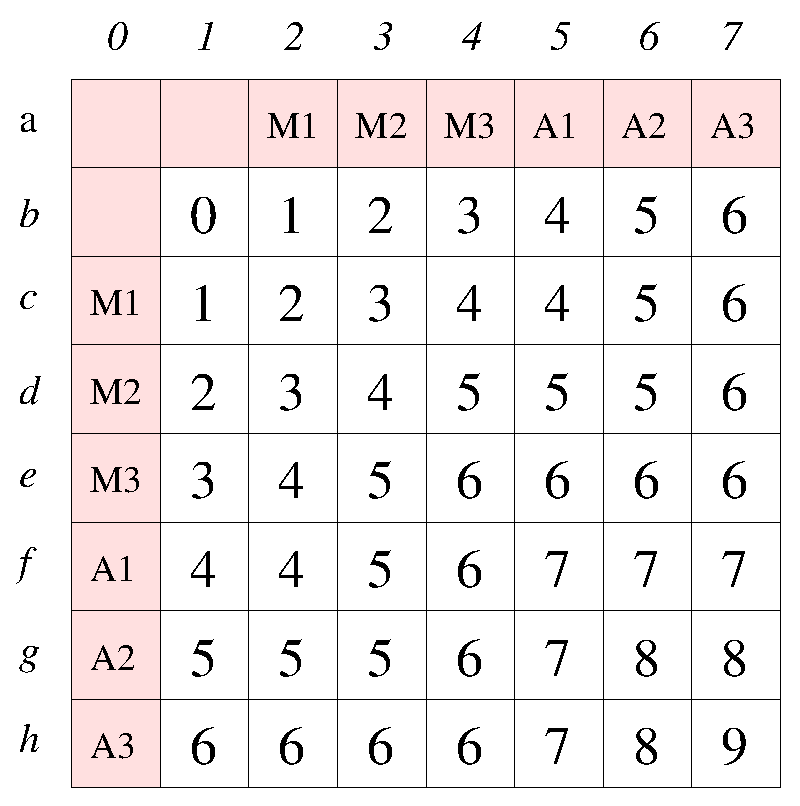
\includegraphics[width=0.3\textwidth]{figs/alloc.eps}
        }
        \hfill
        \subfigure[Stage 2: scoring table filling]
        {
            \label{fig:alloc:2}
            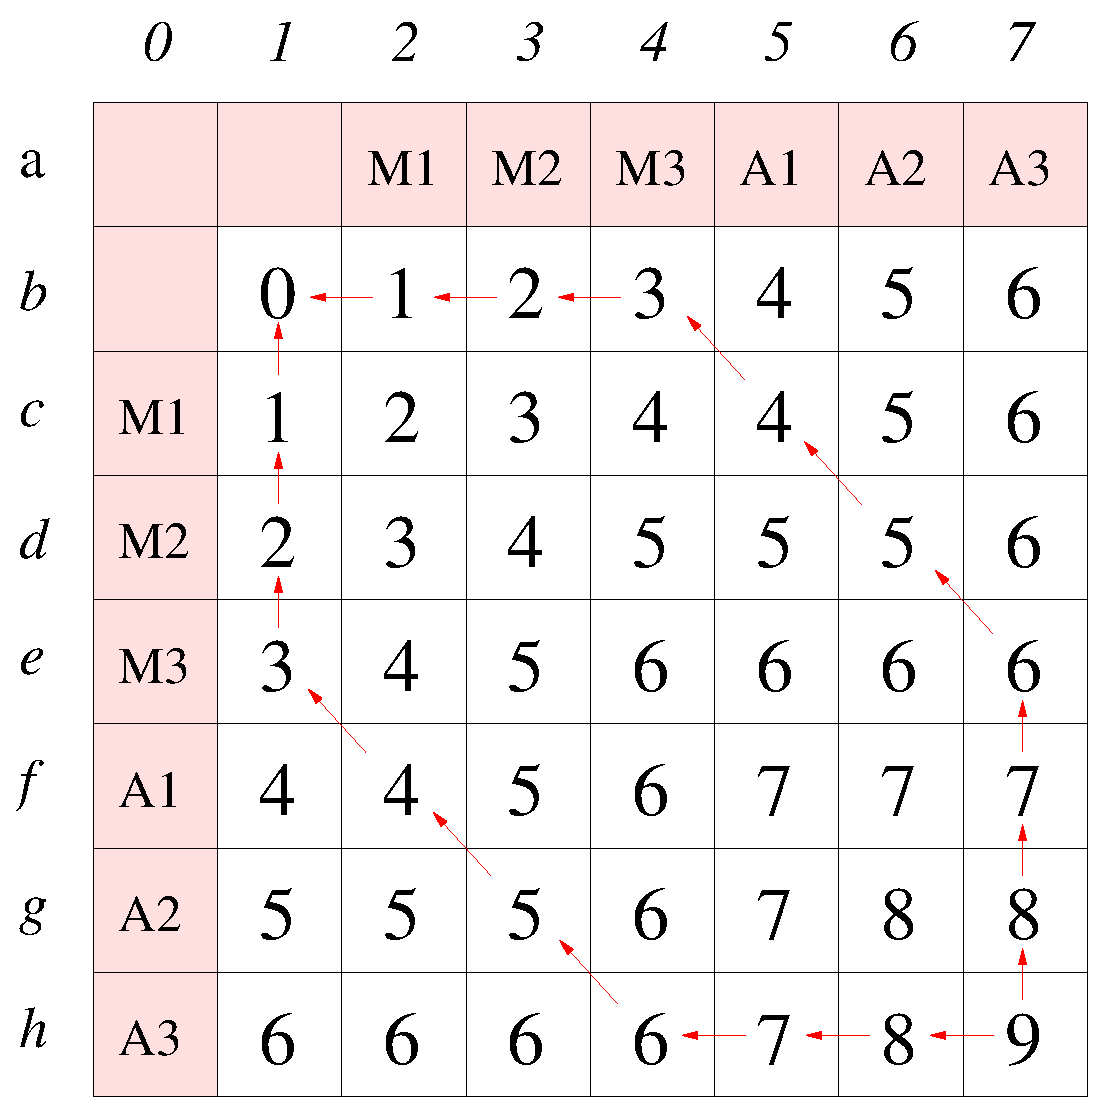
\includegraphics[width=0.3\textwidth]{figs/alloc2.eps}
        }
        \hfill
        \subfigure[Stage 3: backtracking]
        {
            \label{fig:alloc:3}
            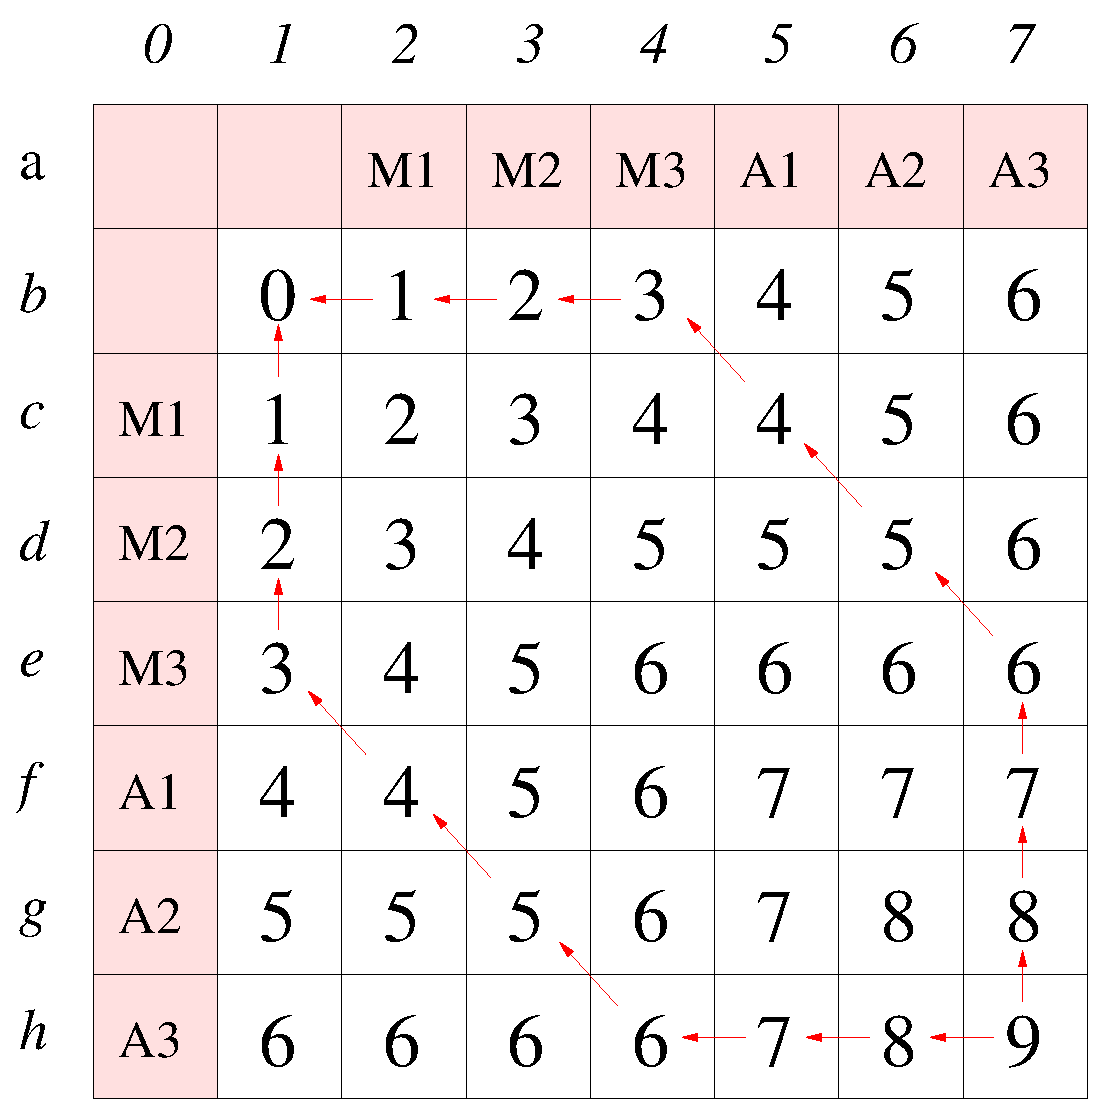
\includegraphics[width=0.3\textwidth]{figs/alloc3.eps}
        }
    \end{center}
    \caption{DP-based ALUs allocation}
    \label{fig:alloc}
\end{figure}
\indent
Lastly, the key to achieving minimum stack consumption is the manipulation of HFPT-sort.
Fig.~\ref{fig:hfpt} shows an example of performing the HFPT-sort on a $bt$, 
where the number in each $sn$ denotes the execution order, 
and each parent receives the first operand from the stack and the second one from the forwarding network.
The postorder-traversal ensures that children are processed before their parent, 
and thus operands received by parents are validated. 
Conventionally, the left-subtree has the priority in the postorder-traversal, 
but we apply the higher-subtree-first rule instead, 
which indicates the higher subtree root has the higher execution priority over its sibling.
This implies that the stack is always used by the higher subtree root.
As a result, for any $bt$, we can represent the stack size requested by HFPT (HFPTSS) in a recursive form:
\begin{equation*}
    HFPTSS(bt) = max(\ HFPTSS(bt.higher\_subtree),\ HFPTSS(bt.lower\_subtree) + 1\ )
\end{equation*}
Based on the equation above, one can use mathematical induction to prove that the stack memory consumes by HFPT is less than or equal to any possible traversal.
%Next, we would like to prove that $HFPTSS(bt)$ is the optimized stack size (OSS) for a $bt$ by mathematical induction, or:
%\begin{equation}
%    HFPTSS(bt) = OSS(bt) 
%\end{equation}
%Letting $bt_n$ denotes a binary tree having a height of $n$, 
%Eq.~4.2 holds apparently for $bt_0$, 
%which forms the basis of methematical induction:
%\begin{equation}
%    HFPTSS(bt_0) = 0 = OSS(bt_0) 
%\end{equation}
%Using the induction hypothesis that the Eq.~4.2 also holds for $bt_k$ and $bt_x$, 
%which are the higher and lower subtrees of $bt_{k+1}$ respectively (i.e., $x < k$), we have:
%\begin{equation}
%    \begin{aligned}
%        HFPTSS(bt_{k+1}) & = max(\ HFPTSS(bt_k),\ HFPTSS(bt_x) + 1\ ) \\
%                         & = max(\ OSS(bt_k),\ OSS(bt_x) + 1\ ) \ \ \text{where } OSS(bt_k) \geq OSS(bt_x) \\
%    \end{aligned}
%\end{equation}
%and the lifetime of data in the stack always correspond to the size of the lower subtree.
%As a result, the lifetime of data in the stack reduced, 
%and the stack consumption is minimized.
%and the higher-first policy ensures that the child of the higher subtree is listed in front of its sibling, 
%which minimizes the lifetime of data in the stack.
\begin{figure}[!h]
    \begin{center}
        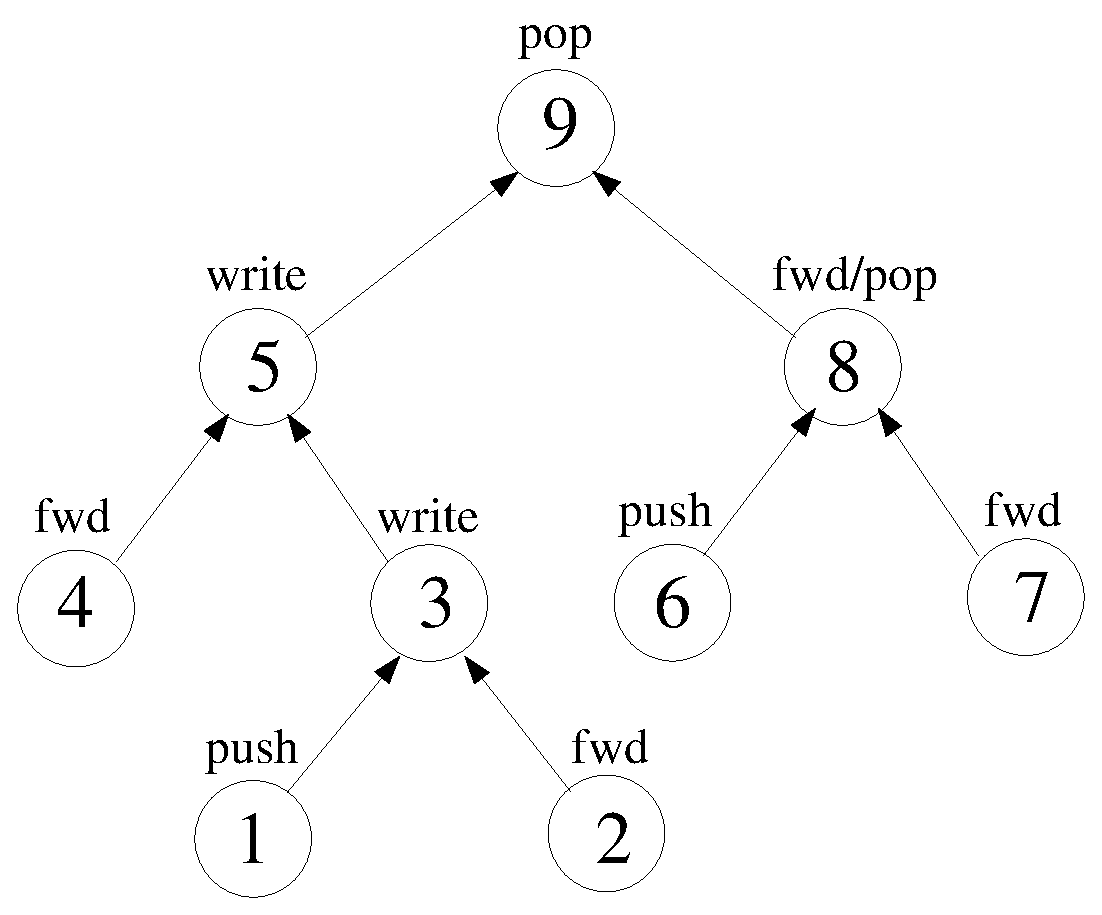
\includegraphics[width=0.45\textwidth]{figs/hfpt.eps}
    \end{center}
    \caption{HFPT-sort}
    \label{fig:hfpt}
\end{figure}%
